\documentclass{article}
\usepackage[utf8]{inputenc}
\usepackage{hyperref}
\usepackage[letterpaper, portrait, margin=1in]{geometry}
\usepackage{enumitem}
\usepackage{amsmath}
\usepackage{amsthm}
\usepackage{booktabs}
\usepackage{graphicx}
\usepackage{float}
\usepackage{hyperref}
\usepackage[flushleft]{threeparttable}
\usepackage{textcomp}
\usepackage{amssymb}
\usepackage{dsfont}
\hypersetup{
colorlinks=true,
    linkcolor=black,
    filecolor=black,      
    urlcolor=blue,
    citecolor=black,
}
\usepackage{natbib}
\usepackage{yhmath}

\usepackage{titlesec}
\bibliographystyle{chicago}
\newcommand{\bib}{references.bib}
\newcommand\iid{\stackrel{\mathclap{iid}}{\sim}}
\newcommand\asym{\stackrel{\mathclap{a}}{\sim}}
\newcommand\convprob{\xrightarrow{p}}
\newcommand\convdist{\xrightarrow{d}}
\newcommand{\N}{\mathbb{N}}
\newcommand{\Z}{\mathbb{Z}}
\newcommand{\E}{\text{E}}
\newcommand{\V}{\text{Var}}
\newcommand{\Av}{\text{Avar}}
\newcommand{\se}{\text{se}}
\newcommand{\corr}{\text{Corr}}
\newcommand{\cov}{\text{Cov}}
\newcommand{\norm}{\text{Normal}}
\newcommand{\indep}{\perp \!\!\! \perp}

\begin{document}
% The tex content below is similar to the given main.tex
 
\title{Homework 7}
\author{Environmental Economics II\\
Maghfira Ramadhani}
\date{\today}
\maketitle

\section*{Problem 1 Python}
\begin{enumerate}
    \item It might not be a sharp RD as vehicle sold in 2017 might be from previous inventory that is produced when the policy is not in place.
    \item Scatter plot of the data is shown in Figure \ref{f1:scatter_plot}. The plot shows that there is a discontinuity at the cutoff point.
    \begin{figure}[H]
        \centering
        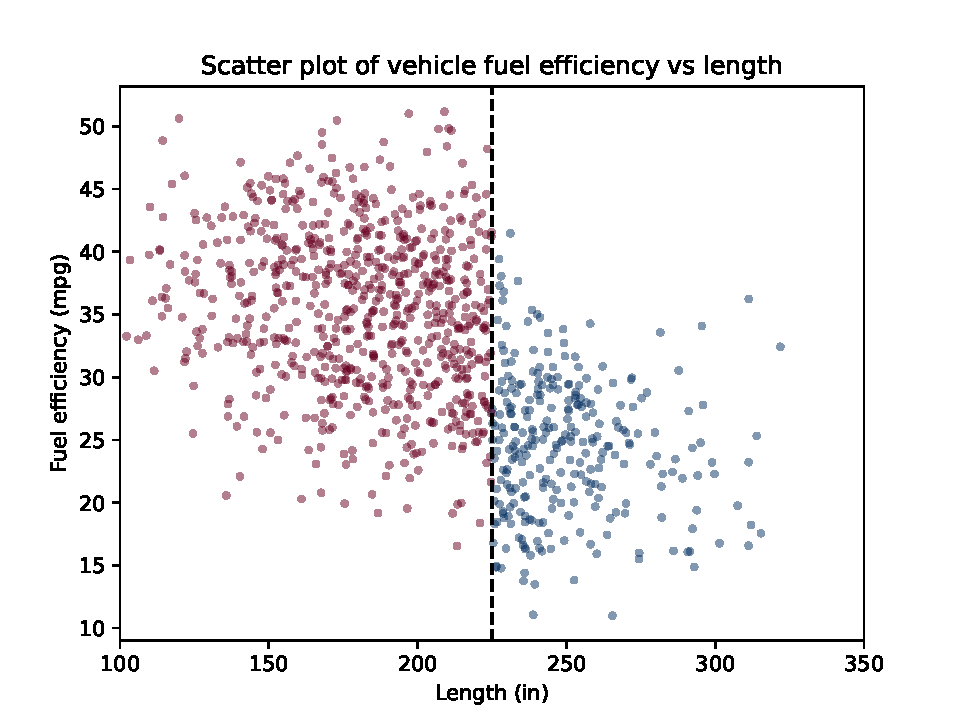
\includegraphics[width=0.4\textwidth]{./figure/scatterplot.pdf}
        \caption{Scatter plot of fuel efficiency vs length of vehicle}
        \label{f1:scatter_plot} 
    \end{figure}
    \item Table \ref{t:RD} shows the RD estimates for using different polynomial.
    \begin{table}[H]\centering
        \caption{RD estimates}
        \label{t:RD}
        \begin{threeparttable}
        \begin{tabular}{@{\extracolsep{5pt}}lccc}
\\[-1.8ex]\hline
\hline \\[-1.8ex]
& \multicolumn{3}{c}{\textit{Dependent variable: Fuel efficiency (mpg)}} \
\cr \cline{2-4}
\\[-1.8ex] & (1) & (2) & (3) \\
\hline \\[-1.8ex]
 LATE & -10.920$^{**}$ & -8.255$^{}$ & 0.376$^{}$ \\
& (4.495) & (46.302) & (0.342) \\
\hline \\[-1.8ex]
 Polynomial specification & 1$^{st}$ order & 2$^{nd}$ order & 5$^{th}$ order \\
 Observations & 1000 & 1000 & 1000 \\
 $R^2$ & 0.399 & 0.399 & 0.401 \\
 Adjusted $R^2$ & 0.397 & 0.396 & 0.395 \\
 Residual Std. Error & 6.158 & 6.160 & 6.165 \\
 F Statistic & 259.649$^{***}$ & 162.427$^{***}$ & 248.217$^{***}$ \\
\hline
\hline \\[-1.8ex]
\textit{Note:} & \multicolumn{3}{r}{$^{*}$p$<$0.1; $^{**}$p$<$0.05; $^{***}$p$<$0.01} \\
\end{tabular}
        \end{threeparttable}
        \end{table}
    The following figure show the resulting first order polynomial.
    \begin{figure}[H]
        \centering
        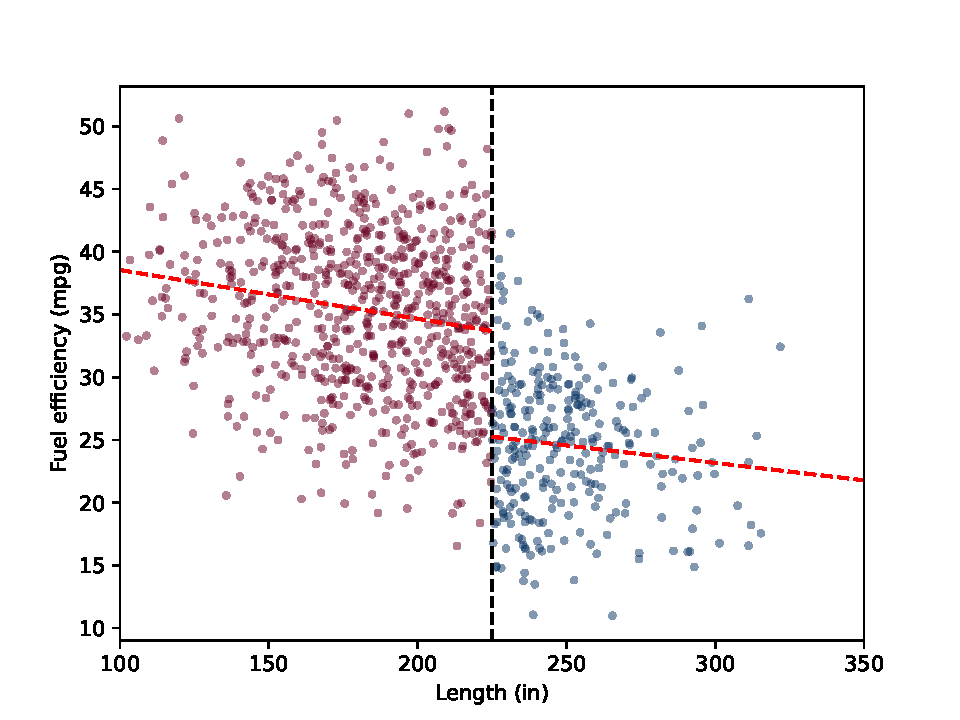
\includegraphics[width=0.4\textwidth]{./figure/RD_1.pdf}
        \caption{RD using first order polynomial}
        \label{f:RD_1} 
    \end{figure}
    \item The following figure show the resulting second order polynomial.
    \begin{figure}[H]
        \centering
        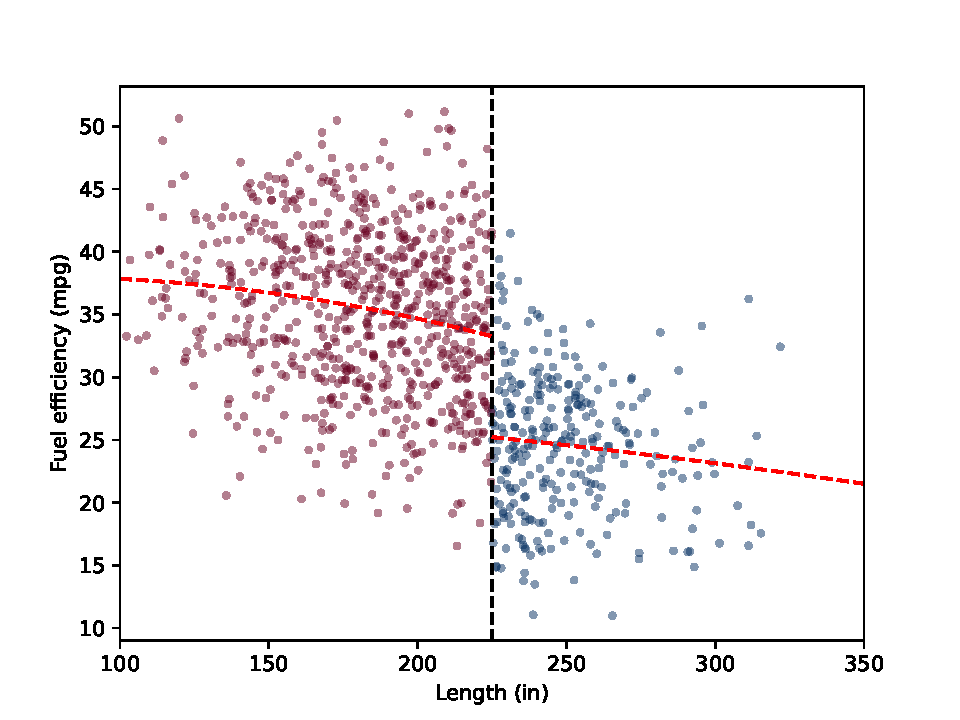
\includegraphics[width=0.4\textwidth]{./figure/RD_2.pdf}
        \caption{RD using second order polynomial}
        \label{f:RD_2} 
    \end{figure}
    \item The following figure show the resulting fifth order polynomial.
    \begin{figure}[H]
        \centering
        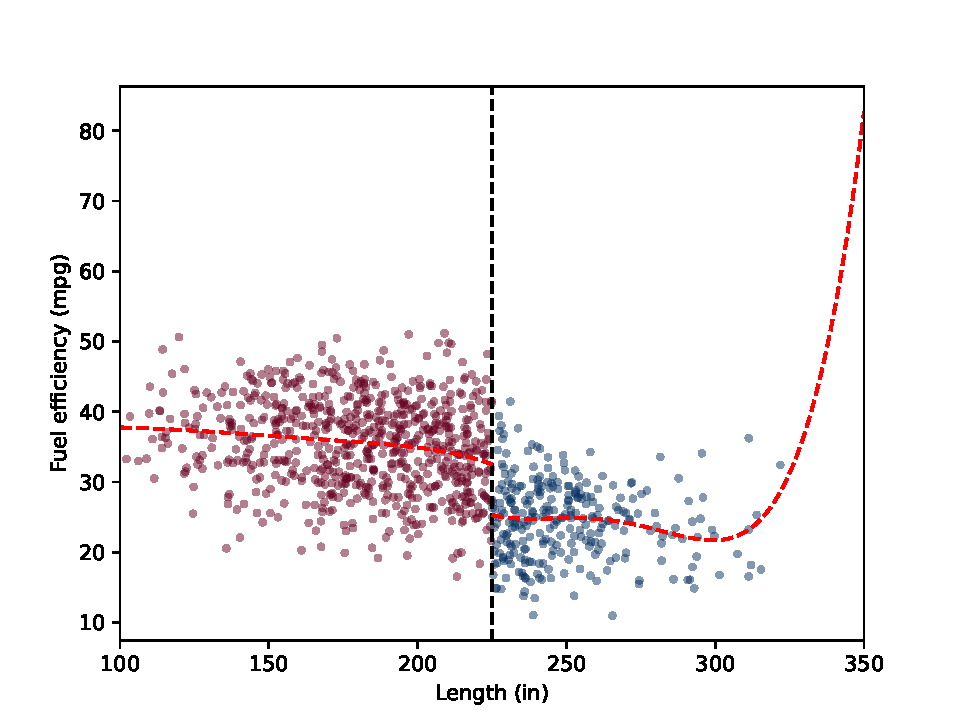
\includegraphics[width=0.4\textwidth]{./figure/RD_3.pdf}
        \caption{RD using fifth order polynomial}
        \label{f:RD_3} 
    \end{figure}
    \item Using the discontinuity as instrument for fuel efficiency, average treatment effect estimate is 158.77 \$/mpg.
\end{enumerate}

\section*{Problem 2 - Stata}
\begin{enumerate}
    \item The LATE from the RD design is -7.9915 with a standard error of 1.2434.
    \begin{enumerate}
        \item The following table shows the second-stage estimates. Note that I did not correct the standard error and directly use the second stage result from Stata. The ATE is 157.43 \$/mpg.
        \begin{table}[H]\centering
            \caption{ATE estimates}
            \label{t:RD_stata}
            \begin{threeparttable}
            \begin{tabular}{l*{2}{c}}
\hline\hline
                    &\multicolumn{1}{c}{Parameter Estimates}&\multicolumn{1}{c}{AME Estimates}\\
\hline
Constant            &      -0.769&            \\
                    &[-1.848,0.310]&            \\
=1 if home received retrofit&       0.904&    -110.729\\
                    &[0.893,0.916]&[-130.589,-90.869]\\
Square feet of home &       0.894&       0.622\\
                    &[0.880,0.909]&[0.607,0.638]\\
Outdoor average temperature (\textdegree F)&       0.281&       2.851\\
                    &[0.039,0.524]&[-2.057,7.758]\\
\hline
Observations        &       1,000&       1,000\\
\hline\hline
\end{tabular}

            \end{threeparttable}
            \end{table}
        \item The plot of the RD is shown in Figure \ref{f:RD_stata}.
        \begin{figure}[H]
            \centering
            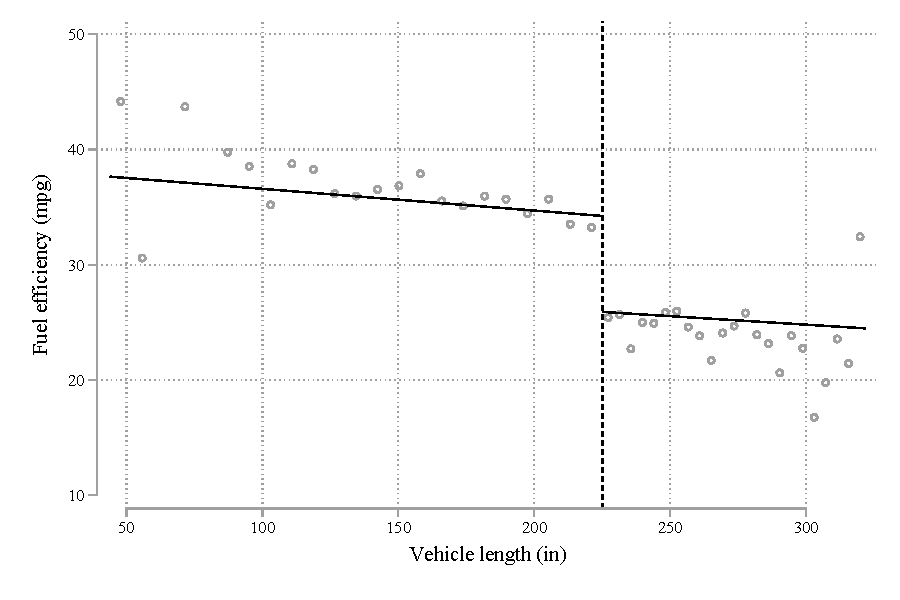
\includegraphics[width=0.5\textwidth]{./figure/RD.pdf}
            \caption{RD using first order polynomial in Stata}
            \label{f:RD_stata} 
        \end{figure}
    \end{enumerate}
    \item abc
\end{enumerate}

\end{document}